\section{Lower Atmospheric Signatures of a Solar Flare Associated with Seismicity}


%\begin{itemize}
%\end{itemize}


\subsection{Background} 
Sunquakes represent the propagation of acoustic waves in the sub-photosphere, responding to an excitation of the photosphere during the impulsive phase of solar flares. The progenitors of sunquakes are thought to be either shocks, radiative backwarming, direct proton collision or sudden magnetic field reconfiguration, see Section \ref{sunprog}. Each of these mechanisms relies on the transport of energy from the corona to the photosphere, and the physical conditions existing in the chromosphere such as magnetic configuration and density. To understand sunquakes and their relationship to solar flares, we need to understand how energy moves down through the solar atmosphere and the physical conditions that are present. 

The majority of the energy released by a flare is deposited in the lower solar atmosphere and manifests itself in the form of enhanced hard X-ray, UV and optical radiation. During the impulsive phase of a solar flare, energy in the form of energetic particles, shocks and MHD waves flow along newly formed coronal magnetic loops, down through the stratified solar atmosphere. As energy is deposited through the differing enviroments of each atmospheric layer, telltale emission signatures are released. 

Hard X-ray (HXR) footpoints are observed due to the excitation of the chromosphere by energetic particle beams accelerated by the reconnecting magnetic field in the the corona during the flare \citep{1995ApJ...455..347A}. According to the standard flare model \citep{1964NASSP..50..451C, 1966Natur.211..695S, 1974SoPh...34..323H, 1976SoPh...50...85K} magnetic reconnection in the corona leads to energy being directed downward in the form of particles, radiation, MHD waves and conduction of heat, which in turn produces ultra-violet (UV) ribbons in the chromosphere. This means that HXR footpoints and UV ribbons observed in the chromosphere directly map to the reconfiguring magnetic fields during the flare. 

As energy moves down through the chromosphere toward the photosphere, emission becomes visible in the optical, termed white light flare (WLF). The processes governing WLF emission in the lower solar atmosphere are detailed by \cite{2007ASPC..368..417D} whereby two main mechanisms are highlighted; Balmer/Paschen continuum emission produced via hydrogen recombination in the lower chromosphere; and enhancement of photospheric continuum emission due to heating of the temperature minimum region. According to \cite{1989SoPh..124..303M}, Balmer/Paschen emission upward (i.e., directly detected) also has a downward component which leads to radiative backwarming of the photosphere. Sunquakes associated with backwarming are likely to be generated by energy deposited by a shock wave formed in the upper-chromosphere or by direct particle collisions with the photosphere. Therefore WLF generation mechanisms are not mutually exclusive and can be expoited as a signature of energy deposition through the lower atmosphere.  



\subsection{Observations}
The X1 flare of the 29th of March 2014 in active region NOAA 12017, was well observed by RHESSI, IRIS and SDO/HMI, collecting HXR, UV and optical emission respectively. The impulsive phase of the flare occurs at 17:46 UT, at which point all mentioned instruments provide good coverage. RHESSI captured hard x-ray data throughout the flare, this data is primarily used to mark the injection site of accelerated energetic particles in the upper-chromosphere. Contour maps of HXRs at energy ranges of 25 - 50 and 50 - 100 keV are aligned with IRIS, SDO/HMI, and acoustic power data to demostrate co-spatial alignment of datasets \ref{saxcontours-vert}. The IRIS spacecraft captured the temporal evolution of the flare between 14:09 and 17:54 UT via it's slit-jaw imager and spectrograph instruments at solar coordinates of 491, 282 arcseconds with a spatial resolution of 0.1667 arcseconds per pixel. The slit-jaw imager data provides coverage of a field of view spanning 167 by 174 arcseconds, of passbands that including 1403, 2796 and 2832 $\AA$. The spectrograph slit is aligned directly over chromospheric flare ribbons, and the sunquake point of origin, providing coverage at central coordinates 491, 282 arcsecinds, with a field of view spanning 14 by 174 arcseconds. The spectrograph slit is exposed for $\sim9$ seconds at 8 slit locations. Wavelengths observed over three channels include FUV1: 1331.7 - 1358.4 $\AA$, FUV2: 1389.0 - 1407.0 $\AA$ and NUV: 2782.7 - 2851.1 $\AA$, associated with the upper-chromosphere down to the upper-photosphere. Spectral lines include C II, Si IV and Mg II h and k. IRIS data is the standard level 2 data product provided for scientific research, which has been calibrated to negate dark currents, flat-field and spacecraft rotational effects. The HMI instrument onboard SDO observed the entire solar photosphere, collecting 6173 $\AA$ continuum intensity data throughout the flare event. HMI has a pixel size of 0.6 arcseconds providing reasonable spatial resolution at a cadence of 45 seconds. HMI data is calibrated to negate cosmic-rays, dark currents, flat-field and spacecraft rotational effects. An 6mHZ acoustic power map, generated via holography techniques, is supplied via private communication by Sergei Zharkova.

\begin{figure}[H]
  \begin{center}
  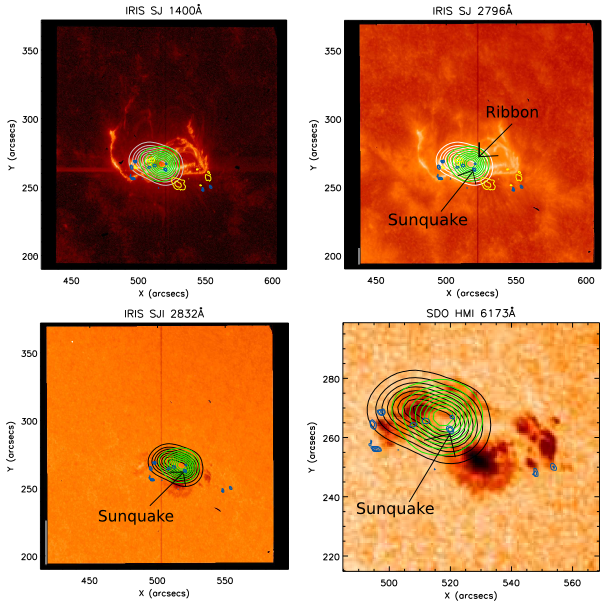
\includegraphics[width=1.0\textwidth]{saxcontours-square}
  \end{center}
  \caption{From top left to bottom right, images represent regions of the solar atmosphere at descending altitudes. The top two and bottom left images show IRIS SJ intensity maps of $1403\AA$ (transition Region), $2796\AA$ (chromosphere), $2832\AA$ (upper-photosphere) data. The bottom right image is SDO HMI $6173\AA$ continuum intensity from the photosphere. Contours show RHESSI HXR with $E = 25-50$ keV in white or black and HXR with $E = 50-100 keV$ in green, sunspot locations in yellow taken from HMI and 6mHz acoustic power in blue.}\label{saxcontours-vert}
\end{figure}


\subsection{Analysis}


White light flares are difficult to see against the bright photospheric background therefore SDO HMI data is subjected to a running difference filter to isolate locations that are white-light enhanced. The running difference filter effectively removes static features leaving behind those pixels that are changing over short time-scales. This is not a perfect process, tending to also highlight granulation features on the photosphere. The next stage is to determine which pixels in the difference image are those that are enhanced during the flare.  These white-light enhanced pixels are identified using a combination of visual inspection and thresholding to eliminate false positives being triggered by noise or granulation features. IRIS SJIs and SG data have no need for filtering.


SJIs of Si IV, Mg II and Mg II wing that are aligned with HMI data and lightcurves are created for pixels at sunquake and ribbon locations. Lightcurves are also created from IRIS spectroscopic data at slit positions aligned with quake and ribbon locations, over a wavelength range of 2825.7 and 2825.8Å within the Balmer continuum which are also aligned with IRIS SJI and HMI data (see Figure \ref{lcseries-bold}). The same IRIS SJ data is converted from DN per pixel to $erg.s^{-1}.cm^{-2}.\AA^{-1}.sr^{-1}$ intensity units, by using recently released conversion factors, which will eventually be used to calculate the amount of energy being deposited in the chromosphere and upper photosphere (see Figure \ref{lcfluxseries}).   

IRIS spectroscopic data are produced at sunquake, ribbon and non-flaring positions (see Figure \ref{spectra}. An egression map of acoustic power  at 6mHz, reveals the position of the sunquake. HXR data from RHESSI and acoustic power data are overlaid on HMI and IRIS slit jaw maps to highlight spatial and temporal evolution of data-sets (see \ref{saxcontours-vert}).\\

\begin{figure}%[H]
  \begin{center}
  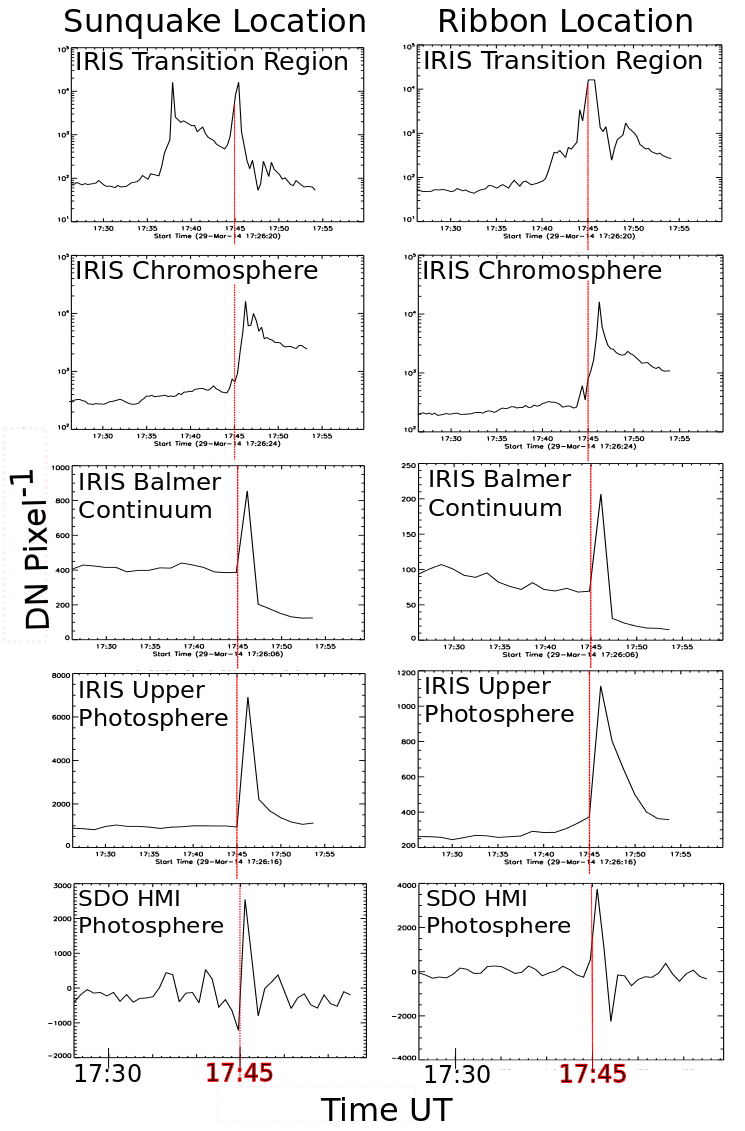
\includegraphics[width=1.0\textwidth]{lcseries-bold}
  \end{center}
  \caption{Left panel shows data over the quake location, right panel shows data over the ribbon location. From top to bottom, plots show lightcurves from IRIS Si IV, Mg II and Balmer wavelengths, with the bottom panel showing the lightcurve from SDO HMI.}\label{lcseries-bold}
\end{figure}

\begin{figure}%[H]
  \begin{center}
  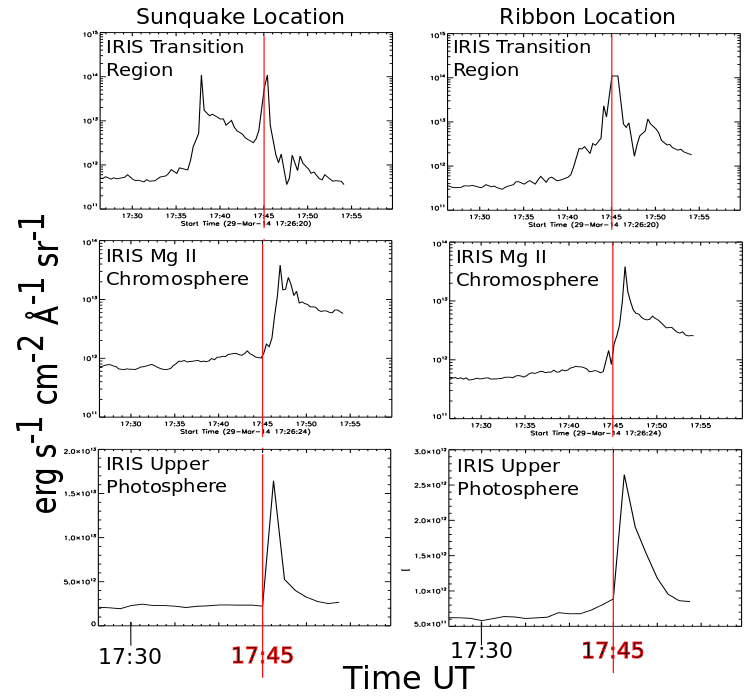
\includegraphics[width=1.0\textwidth]{lcfluxseries}
  \end{center}
  \caption{Left panel shows data over the quake location, right panel shows data over the ribbon location. From top to bottom, plots show lightcurves from IRIS Si IV, Mg II and Balmer wavelengths, with intensity converted into flux units relevent for energy calculations.}\label{lcfluxseries}
\end{figure}

\begin{figure}%[H]
  \begin{center}
  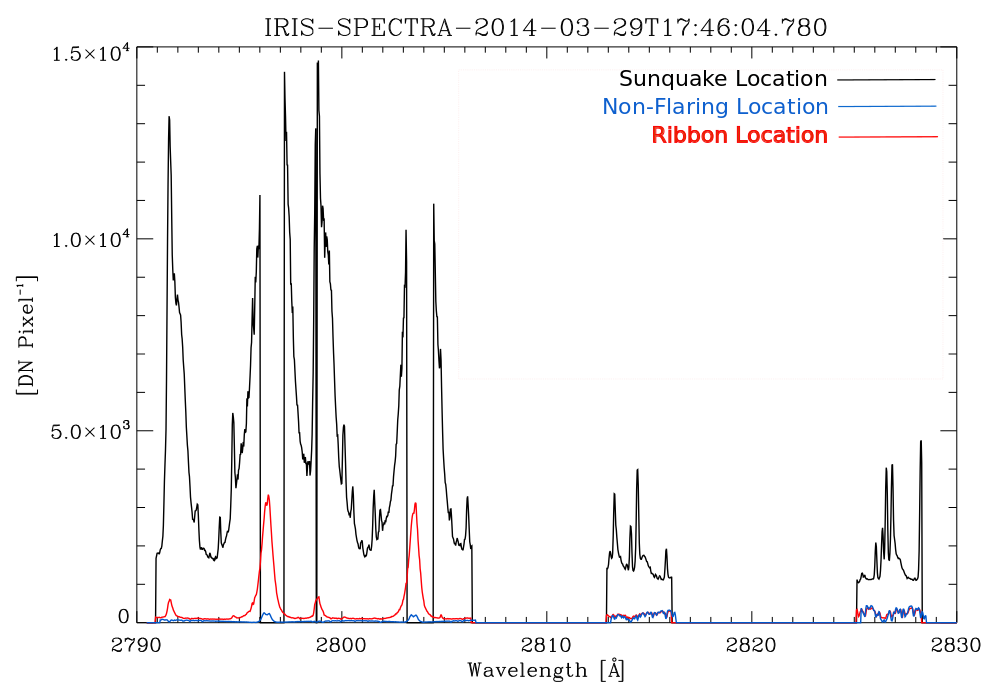
\includegraphics[width=1.0\textwidth]{spectra}
  \end{center}
  \caption{IRIS spectroscopic data ranging in wavelength 2796 - 2830Å with a smaller plot showing a zoom of the region containing the Mg II triplet lines. Black is the spectrum at the quake location (y = 435), red is the spectrum at a point along the ribbon (y = 489) and blue is the spectrum of a non-flaring region (y = 20). Square trough like features represent saturation of the CCD.}
\end{figure}\label{spectra}
 


\subsection{First Results and Discussion}
The location of maximum acoustic power, RHESSI HXR, IRIS and SDO intensity correlate both spatially and temporally \ref{saxcontours-vert}, showing that energy input into the upper chromosphere somehow propagates down to the photosphere. The sunquake is located directly underneath both maximum HXR and white-light emission. 

Intensity lightcurves \ref{lcseries-bold} from SDO and IRIS seem to suggest a similar representation of the movement of energy through the chromosphere to lower altitudes, since their impulsive appearance and peak intensity occur within a minute of each other throughout the different regions. In the transition region above the chromosphere, relative intensity values at both sunquake and ribbon locations increase by three orders of magnitude during the impulsive phase of the flare. The double-peak feature is discussed below. In the chromosphere, relative intensity values at both sunquake and ribbon locations increase by two orders of magnitude during the impulsive phase of the flare. IRIS Balmer light curves for both locations increase by around $100\%$ during the flare indicating the exisitence of radiative backwarming, however, initial values are very different. Pre-flare Balmer emission in the sunquake location is four times that in the ribbon location, this could indicate that radiative backwarming is more prolific above the sunquake, providing a source of further study. Similarly to the Balmer lightcurves, the upper-photosphere data shows the pre-flare sunquake location intensity to be approximately one order of magnitude greater than in the ribbon. Both locations show an order of magnitude increase in relative intensity during the flare. SDO HMI data from the photosphere shows both sunquake and ribbon data-sets display an order of magnitude increase in intensity during the flare, although it seems that the ribbon location has a larger increase.      




IRIS SJI lightcurves converted into $erg.s^{-1}.cm^{-2}.\AA^{-1}.sr^{-1}$ show the emission flux increase during the flare. In the transition region above the chromosphere intensity increases by three orders of magnitude, from $10^11$ to $10^14$ $erg.s^{-1}.cm^{-2}.\AA^{-1}.sr^{-1}$, in both sunquake and ribbon locations. When compared to the ribbon plot, the sunquake location displays an interesting double-peak which seems to suggest that there is a preliminary deposition of energy approximately 7 minutes before the onset of the impulsive phase of the flare. The energy deposited and highlighted by the first of the two peaks could provide a means to lower the density in the upper-chromosphere by causing chromospheric material to expand upward and downward. The resulting downward propagating shock wave could leave an easier path for energy transport during the main flare impulse, allowing penetration to deeper atmospheric layers. This is an idea that will be investigated in more detail in the future. In the chromosphere intensity increases by two order of magnitude, from $10^11$ to $10^13$ $erg.s^{-1}.cm^{-2}.\AA^{-1}.sr^{-1}$, in both sunquake and ribbon locations. In the upper-photosphere intensity increases by one order of magnitude, from $10^12$ to $10^13$ $erg.s^{-1}.cm^{-2}.\AA^{-1}.sr^{-1}$, in both sunquake and ribbon locations. AS described above, pre-flare intensity values differ between the two locations.

Spectroscopic data shown in \ref{spectra} show the sunquake emission to be an order of magnitude greater in amplitude than in the ribbon. The spectrum taken from a non-flaring region is around three orders of magnitude smaller than the sunquake location. This means that the sunquake location is recieving more energy during the flare than both the ribbon an d non-flare locations. Lines over the sunquake location are strongly broadened when compared to spectra elsewhere \ref{spectra} which could indicate heating or increased pressure in these regions. Ribbon and sunquake spectra appear to be redshifted in comparison to the non-flaring region, showing that there must be material moving down through the atmosphere during the flare.\\


\subsection{Future Work}
In the next three to six months the aim is to have completed the following tasks:
\begin{itemize}

\item Calculate energy associated with emission captured by HMI to compare with the acoustic power of the sunquake. 

\item Calculate energy associated with emission captured by IRIS slit jaw and spectrometer in order to estimate energy deposition in the atmosphere. 

\item Calculate energy associated with Balmer emission to assess likely energy contribution of radiative backwarming. 

\item Calculate non-thermal electron power via HXR spectra to estimate the initial energy of the electron beam accelerated by the corona. 

\item A more detailed analysis of IRIS spectroscopic data to estimate velocity, density and temperature of chromospheric material. 

\item Analysis of triplet lines in the wings of Mg II h \& k will be used to determine heating of the lower chromosphere as per recent work by \cite{2015arXiv150401733P}. 

\item Compare spectroscopic data taken by EIS with that of IRIS. 

\item Magnetogram: Look at HMI/SOT data to analyse the configuration of the magnetic field.

\end{itemize}
